\chapter{概览}
\label{cap:overview}
    我们模型的主要目标,就是拿到神经网络的结构,预测该神经网络在特定硬件环境下的运行时间。特别地,我们的模型针对tensorflow框架,也就是说,所有性能数据全部来源于tensorflow,因此,我们的预测结果在其他深度学习框架中不一定能够得到较好的预测结果。另一方面,我们模型主要针对CNN进行设计,能够在现有的广泛使用的CNN网络上有比较好的预测结果,如AlexNet\cite{alexnet}等。我们将工作限制在单机上,对仅CPU、1个GPU、2个GPU、4个GPU环境进行测试建模,得到较为满意的预测性能。
    
\section{模型配置}
    模型的输入部分包括网络的结构或网络对应的数据流图、各个计算模块的参数、运行的硬件平台,共三部分。
    
    网络结构在执行过程中,会先转换为数据流图的形式,这一部分对深度神经网络进行主要的定义。而由于数据流图对输入的形状、维度等没有严格的限制,如图\ref{fig:dag_same}所示。因此,输入部分需要对输入的形状进行预先的定义,以便于之后模型进行模拟调度以及性能预测。
    
    另外,输入需要提供运行的硬件环境,如CPU数量、CPU核心数量、内存大小、GPU型号、GPU显存大小、GPU的数量等。以便模型针对不同硬件环境进行调整。限于资源有限,我们只实现了几个固定环境中的性能模型,因此,现有模型的硬件环境配置只能够调整为固定的几种配置,具体见测试部分,即\ref{cha:eval}章节。

    \begin{figure}[!htbp]
        \centering
        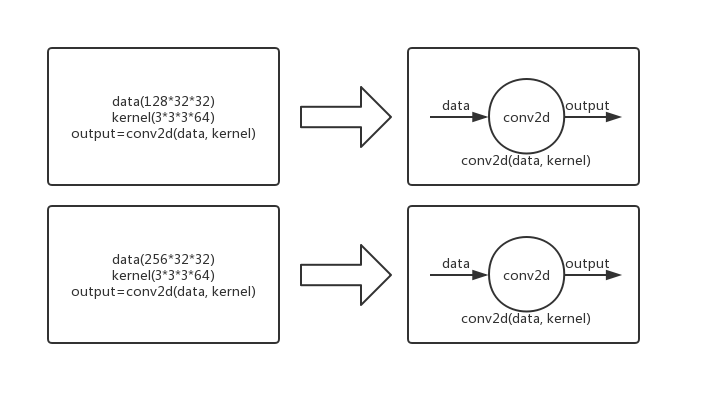
\includegraphics[width=0.8\textwidth]{figures/dag_same.jpg}
        \caption{图中预先定义的两个网络,输入的形状不同,但是生成的数据流图是相同的}
        \label{fig:dag_same}
    \end{figure}
    
\section{模型架构}    
    我们实现的预测模型整体架构如图\ref{fig:arch}所示。主要实现包含两部分,即图中的调度模拟,和性能模型两部分。其中,调度模拟部分根据深度神经网络应用在运行过程中生成的数据流图,模拟预测真实运行情况下每一个操作的运行状况,包括运行的顺序,运行所在设备,运行占用资源等。性能模型部分根据实际Tensorflow中操作运行的时间,建立操作性能模型。得到的结果再提供给调度模拟部分,两部分结合,继而在操作的粒度上,预测在正常的Tensorflow的调度下,深度神经网络应用的运行时间。
    
    \begin{figure}[!htbp]
        \centering
        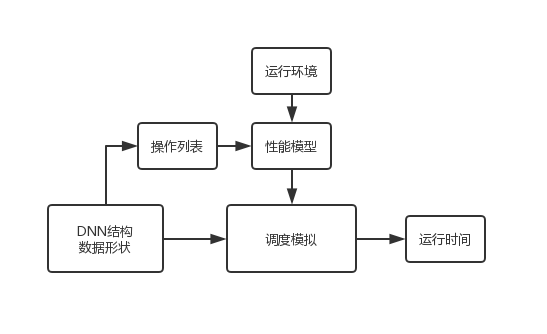
\includegraphics[width=0.8\textwidth]{figures/arch.jpg}
        \caption{预测模型整体架构}
        \label{fig:arch}
    \end{figure}

\subsection{调度模拟}
    TensorFlow中所有的计算任务会被转化为数据流图的形式,其中每个点代表一个计算操作,每一条边表示一组数据。具体到实际运行TensorFlow中,每一个点代表一个计算函数,如矩阵乘法(MatMul)、二维卷积(Conv2D)等,而一条边代表一个张量(tensor)。调度模拟部分的主要工作就是将用户定义的神经网络模型转化为数据流图,并针对数据流图按照tensorflow的方式进行调度。
    
    TensorFlow中,执行计算任务是通过会话(session)的方式进行的,即执行Session.run()命令。在这个过程中,首先进行的是会话的创建,与此同时,将模型转化为数据流图的形式保存。我们的工作主要关注的就是这一步生成的数据流图。而数据流图在创建到运行的过程中,需要经历六个阶段,即图的创建、图的传送、图的剪枝、图的划分、图的二次划分,以及图的运行。下面我将分别对这些部分进行解释。
    
    图的创建,根据用户写入的模型创建数据流图。用户在使用TensorFlow的时候,神经网络是以运算的形式定义的。由于用户的输入为计算任务或数据生成任务,因此,用户的输入均可以直接对应数据流图中的一个子图。以图ref中定义的网络为例,用户定义了两个矩阵,即通过random\_normal操作生成两个$ 1024 \times 1024 $ 的服从正态分布的矩阵$ a $和$ b $。之后定义$ c = a \times b $,$ d = b * c $,最终输出为矩阵$ d $。而在创建图的过程中,输入均被映射到数据流图中的一个子图,其中每个子图都按照对应的任务,对应了一个小的数据流图,用来对定义的运算进行处理。从另一个方向来看,每个计算任务都被先转化成了一个数据流图,再按照用户定义的数据依赖关系组合,就得到了我们创建的数据流图。
    
    图的传送,主要任务是把已经生成好的数据流图序列化,并传送给计算的主机(master)。这一步把之前生成的图(Graph)转化为图定义(GraphDef),再传送给主机(master)。主机(master)是TensorFlow在运行过程中的概念,这一部分与我们的性能预测模型关系不大,因此不做过多介绍。
    
    图的剪枝,根据给定输入与需求输出得到最小依赖子图。主机(master)在得到图定义(GraphDef)后,先进行反序列化转化为原图(Graph),然后根据给定的输入,和需求的输出,对图进行剪枝,具体过程就是进行深度优先搜索(DFS),对图进行标记,从而确定哪些点是得到输出中必要的,并删除其他所有节点和无关的边,将图的规模缩小。
    
    图的划分,把图中的节点分配到不同的机器(worker)上。在Tensorflow中进行多机并行时,需要手动对计算图进行划分,即规定运算所在的机器。在数据并行中,用户需要手动将数据分成若干组,给每一组规定运行的机器。在模型并行中,用户需要规定操作所在的机器。这一步的工作,就是根据用户的输入定义,将图的节点或子图分配到各个机器上。
    
    图的二次划分,把图中节点分配到不同的设备上。机器(worker)根据当前可用的资源,以及用户对操作的约束,将途中的节点分配到不同设备上,如CPU,GPU等。默认情况下,大部分运算操作都会被划分到GPU上。
    
    图的运行,将划分好的节点运行。TensorFlow中执行运算使用StreamExecutor。在图经过两次划分后,对划分好的子图或点进行运行,这一部分TensorFlow会对每个子图启动一个执行器(Executor)实例,用来对这个子图进行运算,StreamExecutor简单来说可以理解成对底层设备的封装,TensorFlow通过StreamExecutor进行执行,可以避免对底层硬件的直接接触。实际运行过程中,如果使用GPU,这里的大部分操作都会被映射为CuBlas函数或CuDNN\cite{cudnn}函数。
    
    调度模拟部分从图的创建开始,进行到图的两次划分为止。由于我们的模型主要运行在单机,因此图的划分这一部分实际均会被划分到同一台机器上。而图的二次划分部分,被放在性能模型部分进行,即对每个操作,根据给定的运行环境,选择不同的模型进行预测。因此,调度模拟部分主要工作就是将用户定义的输入转化为对应的数据流图并剪枝,然后对每个节点调用性能模型。

\subsection{性能模型}
    在卷积神经网络中的推断(inference)过程中,时间占用最长的操作就是Conv2D
